\chapter{Introduction}

This chapter introduces the importance and challenges of data integration, and provides a summary of Semantic Web technologies to demonstrate the feasibility of integrating datasets by instance matching based on ontologies. This chapter also states the motivation and aims of this project to formalise its research focus.


\section{Background}

% Data integration: demand, application, importance, benefits; Ontology matching in data integration;
The ability of using data from multiple sources simultaneously has always been demanded in both research and public areas. For example, translational research data from multiple biomedical domains can be used together to track and analyze human-centered records \cite{DBLP:journals/jbi/WangLFCOHSO09}, and data exported from each peer in its own schema need to be combined in a peer-to-peer (P2P) system \cite{DBLP:conf/dbisp2p/CalvaneseDGLR03}. The process of data integration seeks to identify the semantic interconnections between information from different sources, to promote the seamlessness and effectiveness of operations across multiple datasets in such applications.
\\\\
% The semantic heterogeneity problem of data integration.
Traditional data integration has been problematic due to the semantic heterogeneity problem of datasets, which can be reflected in various aspects. Firstly, the accessibility and usability of data are unpromising, as resources are usually managed by different organisations and stored in different formats such as Excel or scanned PDF, which are not easily readable to computer programmes. In addition, without a formal representation of the semantics of the knowledge within the datasets, computer programmes can only interpret the information at a very basic level \cite{DBLP:journals/expert/ShadboltBH06}, meaning that reasoning about the data can hardly be conducted. Further more, the matching process needs to be carried out even if the datasets come from the same domain of interest, due to the lack of a uniform data modelling principle and a shared vocabulary \cite{euzenat2013d}. Integration of such datasets requires huge amount of extra effort and can sometimes be unrealistic.
\\\\
% Semantic Web foundations and technologies.
The idea of Linked Data and Semantic Web provides a fundamental framework for addressing these issues. Based on the Uniform Resource Identifiers (URIs) \cite{DBLP:journals/rfc/rfc3986} and the HyperText Transfer Protocol (HTTP) \cite{DBLP:journals/rfc/rfc7540} technologies, the idea of Linked Data was formulated so that entities in the world can be uniquely identified by URIs and dereferenced with HTTP. This provides a common way to retrieve entity descriptions from the network \cite{DBLP:journals/ijswis/BizerHB09}. This framework is supplemented by the Resource Description Framework (RDF), which provides a universal, graph-based structure for the data to be modelled, and also to be queried with the SPARQL Protocol and RDF Query Language (SPARQL) \cite{DBLP:journals/tods/PerezAG09}. A shared vocabulary of a knowledge domain can be established as an ontology that is defined in the Resource Description Framework Schema (RDFS) or Web Ontology Language (OWL) \cite{DBLP:journals/expert/ShadboltBH06}, while the entires in one vocabulary can be linked to those in another with RDF triples or OWL axioms \cite{DBLP:journals/ijswis/BizerHB09}. Rules for inference purposes can be specified with the help of Rule Markup Languages (RuleML) \cite{DBLP:journals/entcs/MeiB06}.
\\\\
% Ontology matching.
With the advances of formal knowledge representation with ontologies in the context of Semantic Web, ontology matching techniques have evolved to take advantage of structured domain knowledge and assist in data integration tasks. Information coming from multiple sources are integrated without producing a newly merged dataset. Instead, they are captured by individual ontologies developed to model their respective knowledge domains, and between the ontologies, corresponding classes and instances are linked together to produce an alignment (Figure \ref{fig:align}). This alignment can be used to generate a mediator that can perform various tasks such as data translation, query reformulation and ontology merging \cite{euzenat2013d}, meaning that a query composed over a single dataset can now be reformulated as multiple queries over all the datasets, hence achieving the goal of data integration. This approach has become one of the most recognised solutions to the semantic heterogeneity problem in data integration \cite{DBLP:conf/gil/NafissiBF18}.
\\\\
\begin{figure}[ht]
\begin{center}
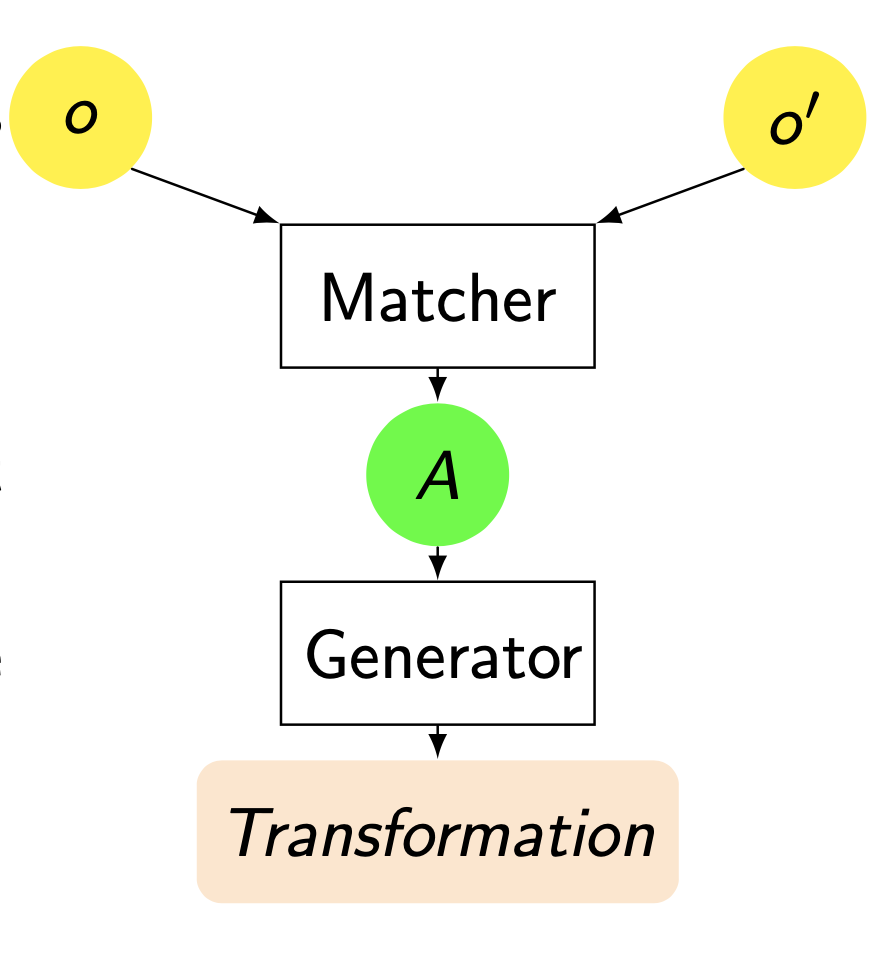
\includegraphics[width=0.3\textwidth]{img/ontomatch.png}
\caption{Alignment production}
\label{fig:align}
\end{center}
\end{figure}
\\\\
% Instance matching.
The general term \textquotedblleft ontology matching\textquotedblright \space involves the matching of both terminological components (TBox), which are related to the classes or concepts, and assertional components (ABox), which are related to the instances or individuals. The concepts of TBox and ABox come from Description Logic (DL) \cite{DBLP:books/daglib/0041477}, which is the mathematical foundation of ontology languages \cite{DBLP:journals/cacm/Horrocks08}. Considering the application in data integration tasks, while the matching of TBoxes (schema-level matching) is important, data are not always presented with proper schema specification \cite{DBLP:conf/boemie/CastanoFMV11}. Further more, the discovery of corresponding instances is necessary for further reasoning on the instance level. This has resulted in a gradual shift of research interests into the instance matching techniques in the recent years, and the introduction of such techniques have shown great achievements and potentials in popular matching systems \cite{DBLP:conf/scdm/AbubakarHMA18}.

% The need of using information simultaneously from multiple sources has been dramatically increasing in the recent researches [? citation] \cite{placeholder}. For example, datasets of different urban infrastructure assets can be integrated to produce a decision support system for city management [heshan], and --- []. Unfortunately, resources are usually constructed and maintained independently in heterogeneous formats [? citation] \cite{placeholder}. The traditional approach of making use of the interdependencies between datasets relies on matching the semantically related entities at the schema level [Ontology matching, 8; Batini et al. 1986; Sheth and Larson 1990; Spaccapietra and Parent 1991; Parent and Spaccapietra 1998] \cite{placeholder}. An obvious drawback of this approach is that updates performed on the individual datasets are not reflected in the merged dataset without extra work. Further more, the matching process needs to be carried out even if the datasets come from the same domain of interest, due to the lack of a uniform modelling principle [ontology matching, 8]\cite{placeholder}.
% \\\\
% Another challenge resides in that the usability of data in the traditional web is usually questionable: datasets can be represented in formats such as CSV, Excel, HTML, PDF table or even scanned pictures [Ontology matching, 11, linked data]. Computers play a very limited role in interpreting such media, doing solely words indexing and document serving, while the intelligent works such as selecting, combining and aggregating the data are performed by human[citation: A Semantic Web Primer, series foreword, xvi].
% \\\\
% The traditional solutions to dataset integration typically relies on matching the semantically related entities at the schema level [Ontology matching, 8; Batini et al. 1986; Sheth and Larson 1990; Spaccapietra and Parent 1991; Parent and Spaccapietra 1998] or the catalog level [Bouquet et al. 2003b, Bernstein and Rahm 2000]. The drawback of such approaches is obvious: updates on the individual datasets are not reflected in the merged dataset without extra work. Further more, the matching process needs to be carried out even if the datasets come from the same domain of interest, due to the lack of a uniform data modelling principle [ontology matching, 8].
% \\\\
% Based on the concept of the semantic web, the research of data integration propose the approach where integration of information coming from multiple local sources is performed without first loading the data into a central warehouse [Chawathe et al. 1994; Wache et al. 2001; Draper et al. 2001; --Halevy et al. 2005--; Seligman et al. 2010; Doan et al. 2012;]\cite{placeholder}. First, a common ontology need to be built as an inter-connection between the ontologies of the domains where the data are sourced from [Ontology matching, 10].
% \\\\
% Description logics (DLs) are a family of knowledge representation languages that can be used to represent knowledge of an application domain in a structured and well-understood way [Citation: An Introduction to Description Logic, 1] \cite{placeholder}. Recently, DLs have played a central role in the semantic web [Hor08], having been adopted as the basis for ontology languages [HPSvH03]. They typically separate domain knowledge into two components: the terminological part TBox and the assertional part ABox, where the combination of a TBox and an ABox is called a knowledge base (KB) [Citation: An Introduction to Description Logic, 1] \cite{placeholder}. A crucial feature of DLs is that terminological and assertional statements have a formal logic-based semantics, meaning that entailments of such statements in a knowledge base can be determined through automated reasoning [Citation: An Introduction to Description Logic, 1] \cite{placeholder}.


\section{Motivation}

A knowledge base typically contains not only a rich schema, but also a large number of instances with enormous assertions about them. For the task of data integration, the alignment of matching instances should be emphasised and produced in a manner that utilises both schema-level and instance-level information. Although a lot of researches have been conducted to propose various kinds of instance matching techniques, most of them do not use sufficient information at the instance level. Specifically, the role axioms that demonstrate properties of relations between individuals, often referred to as the RBox in a description logic context, are often neglected. For example,

\begin{spacing}{1.2}
$$hasMother \sqsubseteq hasParent$$
$$hasParent \sqsubseteq hasAncestor$$
$$Trans(hasAncestor)$$
$$Asym(childOf)$$
$$Disj(hasSibling, childOf)$$
\end{spacing}

are some of the role axioms concerning family relationships that can appear in an ontology.
\\\\
The research focus of this project is to develop an instance matching algorithm that integrates the matching of such role axioms into existing techniques. It is believed that this will benefit the discovery of implicit instance-level knowledge through automated logical reasoning, hence improve the precision and reliability of instance matching for the purpose of data integration.


\section{Aims and Objectives}

The aim of this project is to examine the proposed instance matching idea that integrates the matching of role axioms, by designing and implementing the algorithm to deliver a software tool as a tangible result that can be used for evaluation. In order to achieve this, the following objectives need to be reached:

\begin{spacing}{1.2}
\begin{enumerate}
	\item Study the fundamentals of Semantic Web tachniques and ontology representations.
	\item Explore and manipulate existing strategies for ontology matching and instance matching.
	\item Design the instance matching algorithm to integrate the matching of roles. Analysation of existing approaches will be conducted to facilitate the shaping of the new design.
	\item Implement the design and wrap it in an evaluation framework, to produce a tangible data integration software.
	\item Test and evaluate the implementation, and potentially use description logic reasoners to reason about the implementation.
\end{enumerate}
\end{spacing}

This project is interested in producing the alignment in a fully automatic manner, and tries to avoid manual parameter settings. It should also be noted that it is not the target of the project to achieve complete correctness, which is considered impractical without the aid of domain expert knowledge. However, the level of precision and completeness is still considered as one of the most critical evaluation criterion. The underlying reasonability and decidability of the logic will also be taken into account.


\section{Interim Report Outline}

This chapter has summarised the general background of Semantic Web technologies and the idea of ontology-based instance matching for data integration. The motivation and aims of this project has been stated. Chapter 2 provides a detailed description of previous works related to ontology matching, specifically instance matching, and mentions the most popular matching systems at the present. Chapter 3 justifies the selection of methodologies for the design, and propose a structure of integrating them. Chapter 4 then demonstrates the tools and frameworks used in the implementation steps. Chapter 5 presents the project management and reflections along the progress.
